% -----------------------------------------------------------------
% Document class: Article
\documentclass[ a4paper, twoside, 11pt]{article}
\usepackage{../../../macros-general}
\usepackage{../../../macros-article}
% Number of the handout, quiz, exam, etc.
\newcommand{\numero}{01}
\setcounter{numero}{\numero}

% -----------------------------------------------------------------
\begin{document}
\allowdisplaybreaks

\begin{center}
\Large Mec\'anica Vectorial (MECG-1001): Lecci\'on \numero \\[2ex]
\small \textbf{Semestre:} 2017-2018 T\'ermino II \qquad
\textbf{Instructor:} Luis I. Reyes Castro \qquad
\textbf{Paralelo:} 08
\end{center}
\fullskip

% =============================================
\begin{problem}
Para la armadura mostrada en la siguiente figura (lado izquierdo):
\begin{enumerate}[label=\textbf{\alph*)}]
\item \textbf{3 Puntos:} Utilizando el m\'etodo de las secciones escriba tres ecuaciones de las cuales se puedan resolver para las fuerzas en los miembros $AB$, $AG$ y $FG$. 
\item \textbf{1.5 Puntos:} Calcule las fuerzas en los miembros $AB$, $AG$ y $FG$. Por favor denote fuerzas de compresi\'on con signo positivo y de tensi\'on con signo negativo. 
\item \textbf{3 Puntos:} Utilizando el m\'etodo de las secciones escriba tres ecuaciones de las cuales se puedan resolver para las fuerzas en los miembros $AE$, $AF$ y $EF$. 
\item \textbf{1.5 Puntos:} Calcule las fuerzas en los miembros $AE$, $AF$ y $EF$. 
\end{enumerate}

\end{problem}
\fullskip

% =============================================
\begin{problem}
Para el armaz\'on mostrado en la siguiente figura (lado derecho):
\begin{enumerate}[label=\textbf{\alph*)}]
\item \textbf{2 Puntos:} Bosqueje los diagramas de cuerpo libre de las barras $ABC$ y $DEF$. 
\item \textbf{2 Puntos:} Calcule las fuerzas en los eslabones $AD$ y $BE$. Por favor denote fuerzas de compresi\'on con signo positivo y de tensi\'on con signo negativo. 
\item \textbf{2 Puntos:} Calcule las reacciones en $C$ y $F$. 
\end{enumerate}

\begin{figure}[htb]
\centering
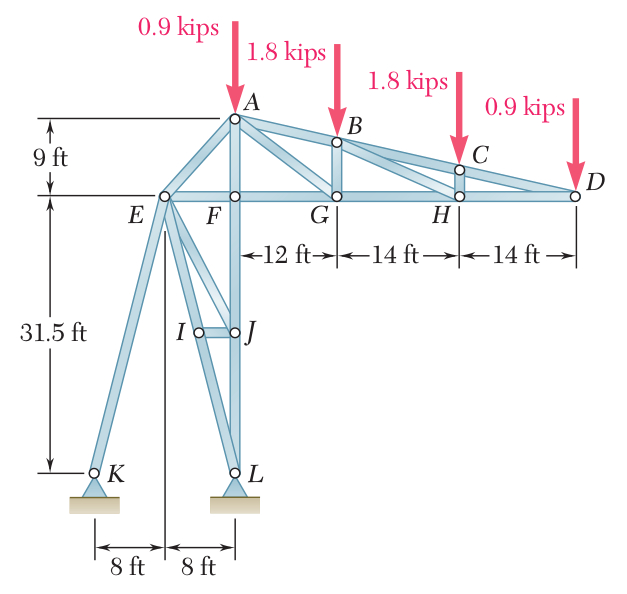
\includegraphics[width=0.56\textwidth]{prob-armadura.jpg} \qquad
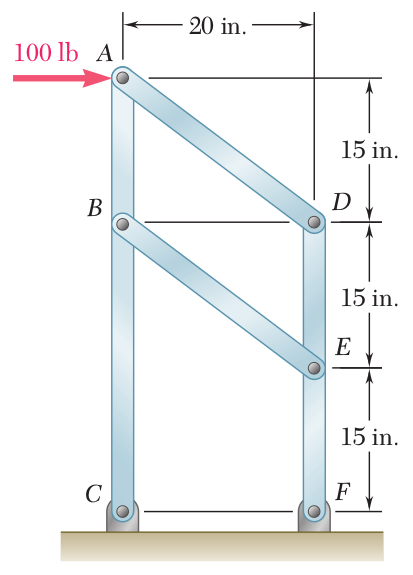
\includegraphics[width=0.32\textwidth]{prob-armazon.jpg}
\end{figure}

\end{problem}
\fullskip

% =============================================
\begin{problem}
Una barra delgada $AB$ de peso $W$ se une a los bloques $A$ y $B$ que se mueven libremente sobre las gu\'ias como se muestra en la siguiente figura. El resorte, que tiene una constante $k$, se encuentra sin deformar cuando $\theta = 0\deg$. 
\begin{enumerate}[label=\textbf{\alph*)}]
\item \textbf{3 Puntos:} Sin tomar en cuenta el peso de los bloques, encuentre una ecuaci\'on en t\'erminos de $W$, $k$, $l$ y $\theta$ que se cumpla cuando la barra est\'a en equilibrio. 
\item \textbf{3 Puntos:} Determine el valor de $\theta$ cuando $W = 75$ lb, $l = 30$ in y $k = 3$ lb/in. 
\end{enumerate}

\begin{figure}[htb]
\centering
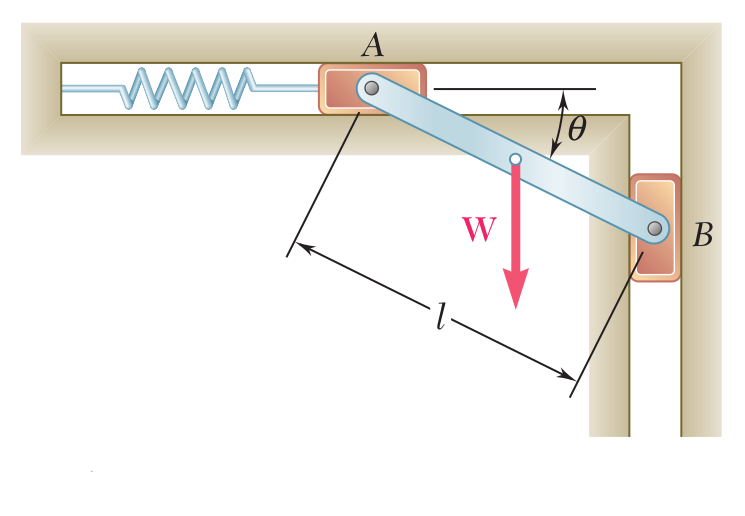
\includegraphics[width=0.42\textwidth]{prob-equilibrio.jpg}
\end{figure}

\end{problem}
\fullskip

% =============================================
\begin{problem}
\textbf{4 Puntos:} Para la viga mostrada en la siguiente figura encuentre la fuerza cortante $V(x)$ y el momento flector $M(x)$ como funci\'on de la posici\'on $x \in [0,4]$. 

\begin{figure}[htb]
\centering
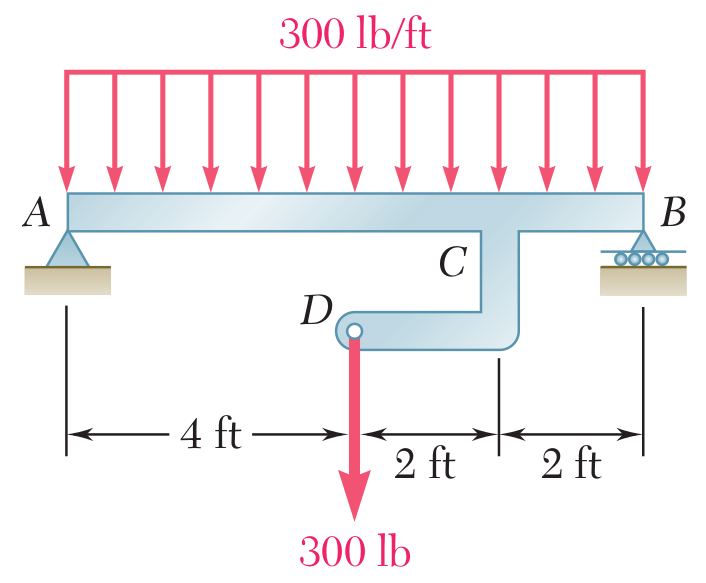
\includegraphics[width=0.36\textwidth]{prob-vigas.jpg}
\end{figure}

\end{problem}
\fullskip

\end{document}